% !TEX TS-program = pdflatex
% !TEX encoding = UTF-8 Unicode

% Author: Michael Wagener

\documentclass[11pt]{article} % use larger type; default would be 10pt

\usepackage{pgf}
\usepackage{tikz}
\usetikzlibrary{arrows,automata,shapes,positioning}
\usetikzlibrary{decorations.pathmorphing} % LATEX and plain TEX when using Tik Z

%\usepackage[simplified]{pgf-umlcd}  % UML-Diagramme
%\usepackage[T1]{fontenc} % https://tex.stackexchange.com/questions/291833/pgf-umlcd-underscore-in-class-name-failing

\usepackage[utf8]{inputenc} % set input encoding (not needed with XeLaTeX)
\usepackage{geometry} % to change the page dimensions
\geometry{a4paper} % or letterpaper (US) or a5paper or....
\geometry{margin=15mm} % for example, change the margins to 2 inches all round
\usepackage[ngerman,english]{babel} % alles auf Deutsch - hier in Englisch!

\usepackage{float}  % https://en.wikibooks.org/wiki/LaTeX/Floats,_Figures_and_Captions
%\floatstyle{boxed} 
\restylefloat{figure}
\usepackage{wrapfig}

\usepackage{booktabs} % for much better looking tables
\usepackage{array} % for better arrays (eg matrices) in maths
\usepackage{paralist} % very flexible & customisable lists (eg. enumerate/itemize, etc.)
\usepackage{verbatim} % adds environment for commenting out blocks of text & for better verbatim
\usepackage{subfig} % make it possible to include more than one captioned figure/table in a single float
\usepackage{scrextend} % für addmargin
\usepackage{listings} % Absatz als Code formatieren
\usepackage{color}
\definecolor{mark}{rgb}{0.8,0.2,0.2} % 1=weiß, 0=schwarz
\definecolor{rowcolor}{rgb}{0.94, 0.97, 1.0}

%\usepackage{hyperref}   % wenn im Inhaltsverzeichnis Links zu den Kapiteln stehen sollen

%\usepackage{soul} % https://alexwlchan.net/2017/10/latex-underlines/

\author{Michael Wagener, JCNS-1}
\title{Internal CrystalScatter program documentation}

\usepackage{fancyhdr} % This should be set AFTER setting up the page geometry
\pagestyle{fancy} % options: empty , plain , fancy
\renewcommand{\headrulewidth}{0pt} % unterdrückt die hor. Linie unter dem Titel
\lhead{}\chead{\textbf{CrystalScatter}}\rhead{\today}
\lfoot{Michael Wagener}\cfoot{\thepage}\rfoot{JCNS-1}

\usepackage{sectsty}
\allsectionsfont{\sffamily\mdseries\upshape} % (See the fntguide.pdf for font help)
% (This matches ConTeXt defaults)

%%% ToC (table of contents) APPEARANCE
\usepackage[nottoc,notlof,notlot]{tocbibind} % Put the bibliography in the ToC
\usepackage[titles,subfigure]{tocloft} % Alter the style of the Table of Contents
\renewcommand{\cftsecfont}{\rmfamily\mdseries\upshape}
\renewcommand{\cftsecpagefont}{\rmfamily\mdseries\upshape} % No bold!

\usepackage{longtable} % Tabellen über mehrere Seiten
\usepackage{multirow} % multirow/multicolumn
\usepackage{colortbl} % farbige Tabellenzellen
%\setlength{\LTpre}{0pt} % Remove whitespace befor and after longtables
%\setlength{\LTpost}{0pt}

\usepackage{tabularx}
\newcolumntype{L}[1]{>{\raggedright\arraybackslash}p{#1}} % linksbündig mit Breitenangabe
\newcolumntype{C}[1]{>{\centering\arraybackslash}p{#1}} % zentriert mit Breitenangabe
\newcolumntype{R}[1]{>{\raggedleft\arraybackslash}p{#1}} % rechtsbündig mit Breitenangabe
\newcommand{\ltab}{\raggedright\arraybackslash} % Tabellenabschnitt linksbündig
\newcommand{\ctab}{\centering\arraybackslash} % Tabellenabschnitt zentriert
\newcommand{\rtab}{\raggedleft\arraybackslash} % Tabellenabschnitt rechtsbündig
% https://de.wikibooks.org/wiki/LaTeX-W%C3%B6rterbuch:_tabular


\setlength{\tabcolsep}{1mm} % Setzt den Längenwert von {Abstand zwischen den Spalten einer Tabelle} auf den Wert 1mm
\setcounter{tocdepth}{2} % Tiefe des Inhaltsverzeichnisses

\begin{document}

\maketitle
\tableofcontents % toc anzeigen

\begin{figure}[b] % die History Tabelle am unteren Seitenrand der ersten Seite anzeigen...
\begin{longtable}{|p{2.7cm}|p{2.6cm}|p{10.3cm}|}
\caption{Document revision history} \\
\hline\rowcolor{rowcolor}{\bf Date} & {\bf Author} & {\bf Short description} \\
\endfirsthead
\hline
April 2023 & M.Wagener & First edit phase. \\ \hline
\end{longtable}

\centerline{All sources saved at https://github.com/neutron-simlab/CrystalScatter}
\end{figure}

\clearpage % neue Seite beginnen


\section{Used source files}

Here are some short informations of what is in each source file. From the history the executable name is {\it sas\_scatter2} but the github name is set to CrystalScatter. This program has a graphical user interface and can calculate one image at a button click. If more images must be calculated, the background process {\it sas\_scatter2Cons} will be used.

{\bf After the big redesign of the gui in April 2023, the background process is not updated at this time. It will be done in the near future.} Then, this remark is removed.

\begin{longtable}{|L{3.6cm}|C{2cm}L{11.5cm}|}
\hline
{\bf sas\_scatter2} & GUI & Main executable. \\ \hline
{\bf sas\_scatter2Cons} & Cons & Background executable, all inputs are provided via parameter and configuration files. \\ \hline
sc\_main.cpp & GUI & The main() function of the main executable. \\ \hline
sc\_mainCons.cpp & Cons & The main() function of the background process. \\ \hline
sc\_maingui.cpp / .h / .ui & GUI & All functions of the gui. \\ \hline
sc\_calcgui.cpp / .h & GUI & Interface from the gui to the calculation class. \\ \hline
%sc\_calcCons.cpp / .h & Cons & Konsolen-Interface zu den Berechnungen \\ \hline
sc\_calc\_generic.cpp / .h & GUI+Cons & Interface class into the calculations. This is historical and might be changed in the future. \\ \hline
sc\_calc\_generic\_gpu.cu / .h & GUI+Cons & Class for the calculations, running on both CPU and GPU. \\ \hline
sc\_libs\_gpu.cu / .h & GUI+Cons & Some routines for the calculations (see note below). \\ \hline
sc\_memory\_gpu.cu / .h & GUI+Cons & Some routines for the memory management on the CPU and GPU (see note below). \\ \hline
sc\_postproc.cpp / .h & GUI+Cons & Image Postprocessing: calculate the (r,phi)-Image and the iFFT. \\ \hline
sc\_simplexfit2d.cpp / .h & GUI+Cons & All functions for the simplex 2d fit algorithm. \\ \hline
sc\_readdata.cpp / .h & GUI+Cons & Functions to read different types of data files. \\ \hline
widimage.cpp / .h & GUI & Class for each image. The images are displayed as separated windows. \\ \hline
dlg*.cpp / .h / .ui & GUI & Dialog functions for some gui features. \\ \hline
myguiparam.cpp / .h & GUI & Helperclass for the parameters. If this will be changed in the future is not known. \\ \hline
\end{longtable}
{\it Note: as a first attempt, I wrote different calculation models in different classes. To have no source duplicates I put all same routines in a library (sc\_libs\_gpu.cu). But it was a problem to compile multiple modules for the gpu with the Qt qmake. So I decide to include the files into the main gpu program. In the future this will be made better...}

The comments in the form ``//Z=number'' are the linenumbers of the corresponding line in the pascal source file from  04.Oct.2022.



\clearpage
\section{The calculation process}

In this chapter I'll describe the process inside the program if the user clicks on the {\it Calculate} Button. This is done in principle also for the simplex 2d fit and in the background process. But here I'll explain only the steps for the main gui.

In the code there are some \#ifdef areas. The meaning and usage is explained in the file sc\_globalConfig.h (unfortunately at the moment in german). In the following explanations I leave these sections out of the descriptions to make it not too complicate to understand.

The user has to fill out all parameters in the gui. If you change the comboboxes some of the other parameters might disappear if they are not needed for this calculation. If you are fine click the {\it Calculate} button. This will start the following routines:

\begin{itemize}
\item SC\_MainGUI::on\_butCalc\_clicked() \\
	Save all parameters to a temporary file. This is done for one reason: if the calculation crashes, you can recover exactly these settings and try some different ones. Then it calls the next function.

\item SC\_MainGUI::local\_butCalc\_clicked() \\
	This procedure is called every time an image must be calculated from the gui (in simplex 2d fit, fft and some test cases). It first calls the preparation (prepareCalculation), then initialize some internal variables for the resulting image size and then starts the calculation (done in a thread!). After the thread is finished some cleanup is done (finishCalculation) and the image will be displayed (addImage).

\item SC\_MainGUI::prepareCalculation( bool progbar ) \\   % bool getMD, 
	This disables some start calculation buttons and enables the progress bar and the abort button. If the parameter getMD is true, all input fields are copied into the calculation class (fillDataFromInputs). After this the preparation inside the calculation class is called (calcGui::prepareCalculation).

\item SC\_MainGUI::fillDataFromInputs() \\
	In the program I use (historically) some hashes/vectors for the variables:
	\begin{itemize}\itemsep0pt
	\item SC\_CalcGUI::inpValues$<$QString,double$>$ used for single value data
	\item SC\_CalcGUI::inpVectors$<$QString,Double3$>$ used for (x,y,z) tupel data
	\item SC\_CalcGUI::inpSingleValueVectors$<$QString,double$>$ are the single values from the tupels above
	\item calcHelper::params$<$QString,paramHelper*$>$ this helper structure contains the values to have no gui access during the calculations and a pointer to the gui element. This might be changed in the future. This hash is filled once in the constructor of the SC\_CalcGUI class.
	\item myGuiParam::allParams$<$myGuiParam*$>$ {\it (vector)} this helper structure contains all parameter informations for each input widget provided in the main calculation tab in the gui.
	\end{itemize}
In this function the common values are copied from the gui input fields into the hashes. All variables are accessed by thier name. The names comes from the first pascal program I've got and represents the variable names there.

\item SC\_CalcGUI::prepareCalculation( bool fromFit ) \\   % , bool getData
	In the normal calculation this calls SC\_Calc\_GENERIC::prepareData( \_dataGetter dg ). From the fit it call the same routine but use another parameter.

\item SC\_Calc\_GENERIC::prepareData( \_dataGetter dg ) \\
	In this procedure all values are copied from the gui elements into the calcHelper::params hash and then put them into the calculation class (into internal variables there). The function provided by the parameter gets two arguments: one string as the name of the parameter and a special value structure to get back all types of values (double, int, bool).

\item myCalcThread::run() \\
	This thread function calls the calculation procedure (SC\_CalcGUI::doCalculation). This is done inside a thread to prevent the gui to freeze.

\item SC\_CalcGUI::doCalculation( int numThreads ) \\
	This calls the real calculation procedure. This step in between was done from the first implementation, there was one pointer to the current class. This will be changed.

\item SC\_Calc\_GENERIC::doCalculation( int numThreads ) \\
	The second intermediate function call.

\item SasCalc\_GENERIC\_calculation::doCalculation( int numThreads ) \\
	In this procedure first a preparation function is called and then the subthreads for the pixel calculations are startet on the CPU (parameter numThreads$>$0) or the GPU (numThreads==0).

\item SasCalc\_GENERIC\_calculation::prepareCalculation() \\
	This procedure runs allways on the CPU because here only the factors are calculated. This is very fast.

\item SasCalc\_GENERIC\_calculation::doThreadCalculation(void *arg) {\it cpu} \\
	This is called in the subthread to convert the thread parameter to the ihex pixel index. Then loop over the other dimension of the image and call the doIntCalc\_GENERIC\_F() routine for calculation.

\item SasCalc\_GENERIC\_calculation::doIntCalc\_GENERIC\_F( CALC, ihex, i ) {\it cpu,gpu} \\
	The values ihex and i are the indices in the image. From these indices and some global parameters the current qx, qy, qz values are calculated. Then the real calculation function (doIntCalc\_GENERIC\_q\_xyz) is called. The CALC variable is the reference to the static SasCalc\_GENERIC\_calculation class to get access to all global variables.

\item SasCalc\_GENERIC\_calculation::doIntCalc\_GENERIC\_q\_xyz(...) {\it cpu,gpu} \\
	This function calculates one pixel value and returns it. The calling function will store this value into the destination array.

\item The following routines are slightly modified for the simplex 2d fit algorithm: \\
	SC\_Calc\_GENERIC::doFitCalculation( int numThreads ) \\
	SasCalc\_GENERIC\_calculation::doThreadFitCalculation(void *arg) \\
	SasCalc\_GENERIC\_calculation::doIntFitCalc\_GENERIC\_F( CALC, ihex, i )

\item SC\_MainGUI::finishCalculation(bool showtime) \\
	This function is called after all pixel values are calculated and reenables the calculation button and disabled the progress bar and the abort button. Then it saves the calculation time used in the SC\_CalcGUI::inpValues hash.

\item int SC\_Calc\_GENERIC\_calculation::minX() \\
	int SC\_Calc\_GENERIC\_calculation::maxX() \\
	int SC\_Calc\_GENERIC\_calculation::minY() \\
	int SC\_Calc\_GENERIC\_calculation::maxY() \\
	These functions returns the dimension if the calculated image. For easier access from the gui, the routines are defined in SC\_CalcGUI and calls internally the above functions in the calculation class.

\item double *SC\_Calc\_GENERIC\_calculation::data() \\
	With this function you get a pointer to the image data. The easier acces is the same as above.

\end{itemize}



%\clearpage
%\section{Ablauf der Berechnungen im Vergleich GUI-Konsole}
%
%Hier der Ablauf / Aufrufe der Funktionen beim Klick auf den Button ``Calc'', dabei werden nur die normalen Berechnungen durchgeführt, also keine FFT! \\
%Aktionen in der GUI $<=>$ Aktionen oder Anmerkungen für die Konsole. \\
%
%void {\bf SC\_MainGUI::on\_butCalc\_clicked()} $<=>$ Aufruf
%\begin{itemize}\itemsep0pt % 1
%\item prepareCalculation( true, true );
%	\begin{itemize}\itemsep0pt % 2
%	\item void {\bf SC\_MainGUI::prepareCalculation( bool getMD, bool progbar )} \\
%		Buttons sperren $<=>$ fällt weg \\
%		current = this; \\
%		fillDataFromInputs(); $<=>$ durch auslesen des Parameterfiles
%		\begin{itemize}\itemsep0pt % 3
%		\item[] void {\bf SC\_MainGUI::fillDataFromInputs()} $<=>$ fällt weg \\
%				Globale Inputs für die Berechnungen aus der GUI füllen \\
%				QHash$<$QString,Double3$>$ SC\_CalcGUI::inpVectors; \\
%				QHash$<$QString,double$>$  SC\_CalcGUI::inpValues; \\
%				QHash$<$QString,double$>$  SC\_CalcGUI::inpSingleValueVectors;
%		\end{itemize} % 3
%	\item[] QString m\_name = ui-$>$tabMethods-$>$tabText(ui-$>$tabMethods-$>$currentIndex()) \\
%		calcGui-$>$prepareCalculation(m\_name,getMD);
%		\begin{itemize}\itemsep0pt % 4
%		\item[] void {\bf SC\_CalcGUI::prepareCalculation( QString m, bool getData )} \\
%			curMethod = methods[m]; \\
%			curMethod-$>$subCalc-$>$prepareData( \&dataGetter ); $<=>$ Callback anpassen
%			\begin{itemize}\itemsep0pt % 5
%			\item {\bf void SC\_Calc\_FCC::prepareData( \_dataGetter dg )} \\
%				\_valueTypes val; \\
%				(*dg)( "RadioButtonQ1", val );  calc-$>$setRadQ1( val.value $>$ 0 ); \\
%				(*dg)( "RadioButtonQ2", val );  calc-$>$setRadQ2( val.value $>$ 0 ); \\
%				...
%			\end{itemize} % 5
%		\end{itemize} % 4
%	\end{itemize} % 2
%\item calcGui-$>$doCalculation( ui-$>$inpNumCores-$>$value(), \&this-$>$myProgressAndAbort );
%	\begin{itemize}\itemsep0pt % 6
%	\item void {\bf SC\_CalcGUI::doCalculation( int numThreads, progressAndAbort pa )} \\
%		curMethod-$>$subCalc-$>$doCalculation( memory, numThreads, pa );
%		\begin{itemize}\itemsep0pt % 7
%		\item[] void {\bf SC\_Calc\_FCC::doCalculation( SC\_GpuMemory *mem, int numThreads, progressAndAbort pa )} \\
%			calc-$>$doCalculation( mem, numThreads, pa ); (im GPU-Code)
%		\end{itemize} % 7
%	\end{itemize} % 6
%\item finishCalculation(true); $<=>$ fällt weg
%	\begin{itemize}\itemsep0pt % 8
%	\item void {\bf SC\_MainGUI::finishCalculation( bool showtime )} \\
%		Buttons wieder freigeben \\
%		calcGui-$>$inpValues.insert( ``\_CalcTime\_'', calcGui-$>$higResTimerElapsed() );
%	\end{itemize} % 8
%\item addImage( false, calcGui-$>$minX(), calcGui-$>$maxX(), calcGui-$>$minY(), calcGui-$>$maxY(), \\
%	 calcGui-$>$data(), ``Image'', true ); $<=>$ Speichern direkt als Image ohne Metadaten
%\end{itemize} % 1


\clearpage
\section{Interfaces}

In this chapter the three interfaces between the gui and the calculation procedures are described:
\begin{itemize}\itemsep0pt
\item variable settings - each variable can be set by their own call
\item group settings - the groups shown in the gui can be set each with one call
\item model settings - here we develop routine call sequences for specialized models
\end{itemize}
In this screenshot all possible parameters are shown. The parameters with grey lables are normally hidden and not used in this selection of the comboboxes.
\begin{figure}[H]
 \centering
 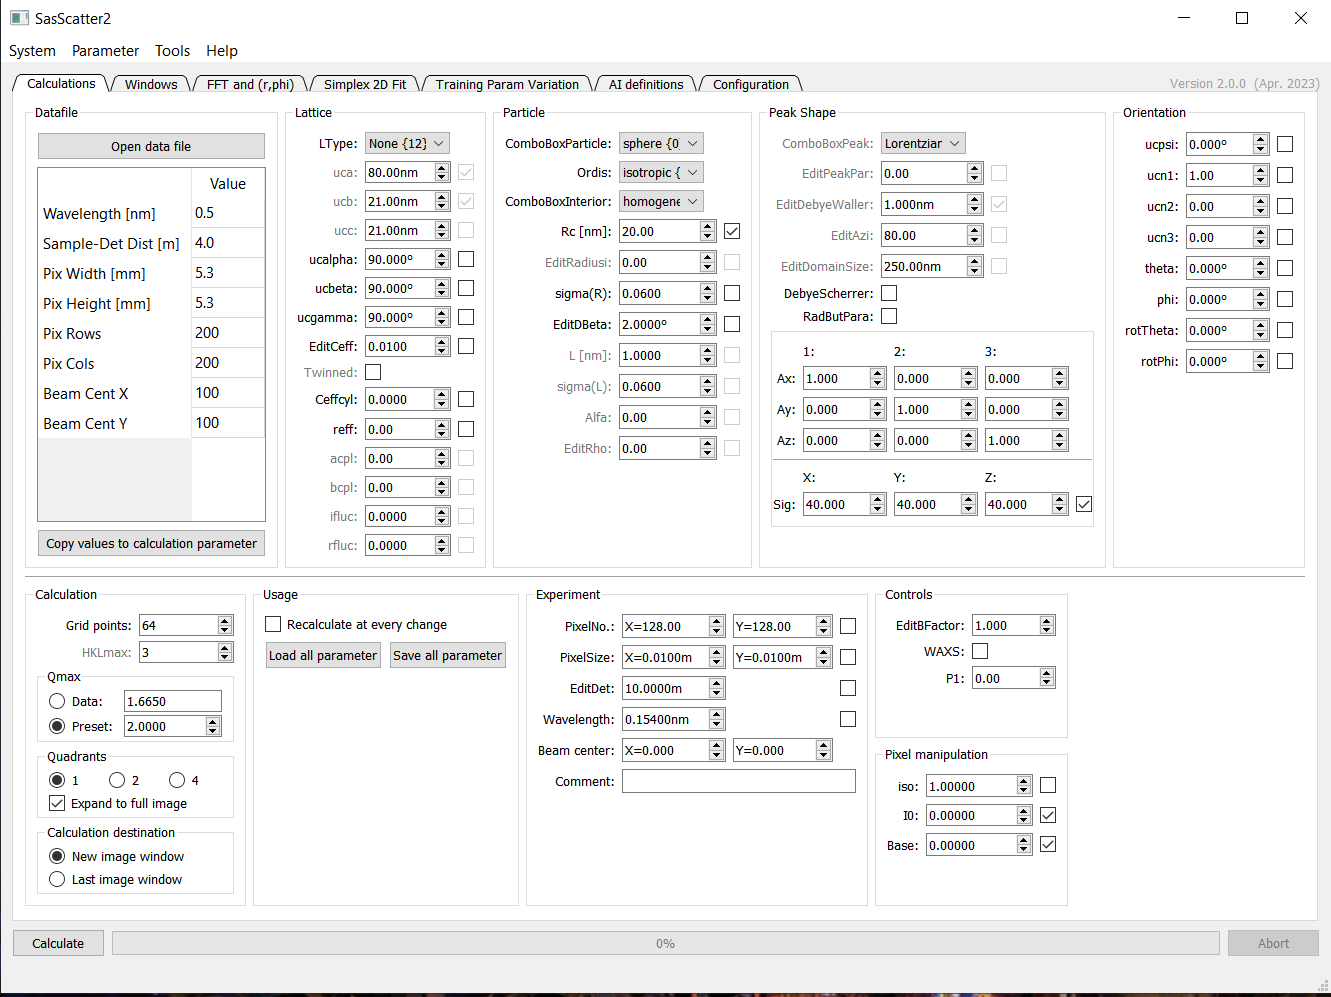
\includegraphics[width=0.99\textwidth]{gui-grouping.png}
 \caption{Calculation parameter grouping with no hidden values.}
\end{figure}

\subsection{Variable settings}

There is one call to each variable. Some variables are converted directly to the correct internal range. There is no range checking done. This must be provided by the gui or the caller.
\begin{itemize}\itemsep0pt
%
\item[] {\it Lattice params}
\item setLType(int ltype) sets the lattice type from the combobox, ltype has a range from 0 to 22.
\item setUCA(double uca) dimension a of the unit cell in nm.
\item setUCB(double ucb) dimension b of the unit cell in nm.
\item setUCC(double ucc) dimension c of the unit cell in nm.
\item setUCalpha(double ucalpha) rotation angle alpha in degrees.
\item setUCbeta(double ucbeta) rotation angle beta in degrees.
\item setUCgamma(double ucgamma) rotation angle gamma in degrees.
\item setCeffF(double editceff)
\item setCheckBoxTwinned(bool twinned)
\item setCeffCyl(double ceffcyl)
\item setReff(double reff)
\item setAcpl(double acpl)
\item setBcpl(double bcpl)
\item setIFluc(double ifluc)
\item setRFluc(double rfluc)
% 
\item[] {\it Particle params}
\item setComboBoxParticle(int cbparticle) sets the particle type and has a range from 0 to 10.
\item setOrdis(int cbordis) sets the ordis value and has a range from 0 to 13.
\item setComboBoxInterior(int cbinterior) this has a range from 0 to 4.
\item setRadiusF(double radius) radius in nm.
\item setRadiusI(double radiusi) second radius in nm.
\item setSigmaF(double sigma)
\item setDBetaF(double dbeta) in degrees.
\item setLength(double length) in nm.
\item setSigmaL(double sigmal)
\item setAlphash(double alpha)
\item setRho(double rho)
% 
\item[] {\it PeakShape params}
\item setComboBoxPeak(int cbpeak) this has a range from 0 to 7.
\item setPeakPar(double peakpar)
\item setDisplacement(double debyewaller) displacement=debyewaller; dwfactor=debyewaller*debyewaller/3.0;
\item setAzi(double azi)
\item setDomainsize(double domainsize)
\item setRadioButtonDebyeScherrer(bool debyescherrer)
\item setRadioButtonPara(bool para)
% 
\item[] {\it PeakShapeMatrix params} \\
	The class {\it Double3} contains x, y and z values.
\item setAx1(Double3) sets ax1, ay1, az1.
\item setAx2(Double3) sets ax2, ay2, az2.
\item setAx3(Double3) sets ax3, ay3, az3.
\item setSigXYZ(Double3) sets sigx, sigy, sigz.
% 
\item[] {\it Orientation params}
\item setUCpsi(double ucpsi)
\item setUCn1(double ucn1)
\item setUCn2(double ucn2)
\item setUCn3(double ucn3)
\item setPolTheta(double theta)
\item setPolPhi(double phi)
\item setRotTheta(double rottheta)
\item setRotPhi(double rotphi)
% 
\item[] {\it Calculation params}
\item setGridPoints(int gridp) defines the dimension (one half of each axis) of the output image
\item setHKLmax(int hklmax) defines the deep of recursions
\item setQMax(double qmax)
\item setRadQ1(bool radq1) \\
	setRadQ2(bool radq2) \\
	setRadQ4(bool radq4) call one of these with true if this quadrant should be calculated. {\it There are three calls because they are callbacks of the radiobuttons in the gui.}
\item setExpandImage(bool expand) set this to true to expand the calculated image to all quadrants.
% 
\item[] {\it Experiment params}
\item setpixnox(double pixelnox) detector pixel count horizontally.
\item setpixnoy(double pixelnoy) detector pixel count vertically.
\item setpixx(double pixelsizex) size of one detector pixel horizontally in m.
\item setpixy(double pixelsizey) size of one detector pixel vertically in m.
\item setdet(double detdist) detector distance in m.
\item setwave(double wavelength) wavelength in nm.
\item setBeamStop(double beamcx, double beamcy) sets the x and y coordinates of the beamstop in pixel indices.
% 
\item[] {\it Control params}
\item setBFactorF(double bfactor)
\item setCheckBoxWAXS(bool waxs)
\item setP1(double p1)
% 
\item[] {\it PixelManipulation params}
\item setIso(double iso)
\item setIZero(double i0)
\item setBase(double base)
\end{itemize}


\subsection{Group settings}

There are calls for almost every group of parameters: Lattice, Particle, Peak Shape with the matrix, Orientation, Calculation with Qmax and Quadrants, Experiment, Controls, Pixel manipulation. The parameter names are the same as above.

\begin{itemize}\itemsep0pt
\item {\bf setLatticeParams}(int ltype, double uca, double ucb, double ucc,
                          double ucalpha, double ucbeta, double ucgamma,
                          double editceff, bool twinned, double ceffcyl,
                          double reff, double acpl, double bcpl,
                          double ifluc, double rfluc)
\item {\bf setParticleParams}(int cbparticle, int cbordis, int cbinterior,
                           double radius, double radiusi, double sigma,
                           double dbeta, double length, double sigmal,
                           double alpha, double rho)
\item {\bf setPeakShapeParams}(int cbpeak, double peakpar, double debyewaller,
                            double azi, double domainsize, bool debyescherrer,
                            bool para)
\item {\bf setPeakShapeMatrix}(double ax1, double ax2, double ax3,
                            double ay1, double ay2, double ay3,
                            double az1, double az2, double az3,
                            double sigx, double sigy, double sigz)
\item {\bf setOrientationParams}(double ucpsi, double ucn1, double ucn2, double ucn3,
                              double theta, double phi, double rottheta, double rotphi)
\item {\bf setCalculationParams}(int gridp, int hklmax, double qmax, bool radq1,
                              bool radq2, bool radq4, bool expand)
\item {\bf setExperimentParams}(double pixelnox, double pixelnoy, double pixelsizex,
                             double pixelsizey, double detdist, double wavelength,
                             double beamcx, double beamcy)
\item {\bf setControlParams}(double bfactor, bool waxs, double p1)
\item {\bf setPixelManipulationParams}(double iso, double i0, double base)
\end{itemize}


\subsection{Model settings}

This part is still under development. If you want to extract sone code pieces to write your own implementation, please ask for the correct statements.

\subsubsection{Spheres}

If you want a simple sphere model for the sample, you can extract some code and implement your own routines (see below) or you can call some of the above routines and get the resultant image from this package. Here is a list of routines to be called with some parameter settings for the result. Bold parameter names denotes the values you have to specify, here are the values for the image shown below.
\begin{itemize}
\item group parameter calls
\begin{itemize}\itemsep0pt
\item setLatticeParams(ltype=12, uca=1, ucb=1, ucc=1, ucalpha=0, ucbeta=0, ucgamma=0, editceff=0.01, twinned=false, ceffcyl=0, reff=0, acpl=0, bcpl=0, ifluc=0, rfluc=0)
\item setParticleParams(cbparticle=0, cbordis=7, cbinterior=0, {\bf radius}=16.7, radiusi=0, {\bf sigma}=0.0639, dbeta=0, length=0, sigmal=0, alpha=0, rho=0)
\item setPeakShapeParams(cbpeak=7, peakpar=0, debyewaller=0, azi=0, domainsize=0, debyescherrer=false, bool para=false)
\item setPeakShapeMatrix(ax1=1, ax2=0, ax3=0, ay1=0, ay2=1, ay3=0, az1=0, az2=0, az3=1, sigx=40, sigy=40, sigz=40)
\item setOrientationParams(ucpsi=0, ucn1=1, ucn2=0, ucn3=0, theta=0, phi=0, rottheta=0, rotphi=0)
\item setCalculationParams({\bf gridp}=128, hklmax=1, {\bf qmax}=2, radq1=false, radq2=false, radq4=true, expand=false)
\item setExperimentParams({\bf pixelnox}=128, {\bf pixelnoy}=128, {\bf pixelsizex}=0.0025, {\bf pixelsizey}=0.0025, {\bf detdist}=10, {\bf wavelength}=0.154, {\bf beamcx}=0, {\bf beamcy}=0)
\item setControlParams(bfactor=0.01, waxs=false, p1=0)
\item setPixelManipulationParams(iso=0, i0=1, base=0)
\end{itemize} % group

\item single value calls
\begin{itemize}\itemsep0pt
\item setLType(ltype=12)
\item setComboBoxParticle(cbparticle=0)
\item setOrdis(cbordis=7)
\item setComboBoxInterior(cbinterior=0)
\item setRadiusF({\bf radius}=16.7)
\item setSigmaF({\bf sigma}=0.0639)
\item setRadioButtonDebyeScherrer(debyescherrer=false)
\item setRadioButtonPara(para=false)
\item setAx1(Double3(1,0,0))
\item setAx2(Double3(0,1,0))
\item setAx3(Double3(0,0,1))
\item setSigXYZ(Double3(40,40,40))
\item setUCpsi(ucpsi=0)
\item setUCn1(ucn1=1)
\item setUCn2(ucn2=0)
\item setUCn3(ucn3=0)
\item setPolTheta(theta=0)
\item setPolPhi(phi=0)
\item setRotTheta(rottheta=0)
\item setRotPhi(rotphi=0)
\item setGridPoints({\bf gridp}=128)
\item setQMax({\bf qmax}=2)
\item setRadQ4(radq4=true)
\item setExpandImage(expand=false)
\item setpixnox({\bf pixelnox}=128)
\item setpixnoy({\bf pixelnoy}=128)
\item setpixx({\bf pixelsizex}=0.0025)
\item setpixy({\bf pixelsizey}=0.0025)
\item setdet({\bf detdist}=10)
\item setwave({\bf wavelength}=0.154)
\item setBeamStop({\bf beamcx}=0, {\bf beamcy}=0)
\item setBFactorF(bfactor=0.01)
\item setCheckBoxWAXS(waxs=false)
\item setP1(p1=0)
\item setIso(iso=0)
\item setIZero(i0=1)
\item setBase(base=0)
\end{itemize}
\end{itemize}
Then a call to doCalculation() starts the calculations and you can retrieve the result with the data() pointer. With the above settings you will get this image:
\begin{figure}[H]
 \centering
 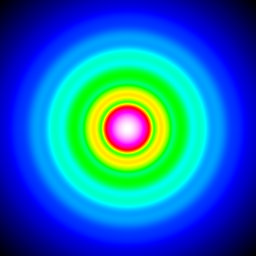
\includegraphics[width=0.4\textwidth]{Vitess-Sphere.png}
 \caption{Example sphere image.}
\end{figure}

\clearpage
If you want to extract the source code for the same result, then you can use the following parts. The values provided as inputs are written in capital letters and the code presented here is cleaned up a little bit.
\begin{itemize}
\item First you have to calculate the coefficients. This is done in sc\_calc\_generic\_gpu.cu in the routine SasCalc\_GENERIC\_calculation::coefficients() and is called only once for each image: \\
{\it Inputs:} RADIUS{\small =16.7}, SIGMA{\small =0.0639} from the user/experiment \\
{\it Inputs:} dim=3=sphere, cs=0=homogeneous from the gui
 % , xleftmargin=0.1cm, xrightmargin=0.1cm
\begin{lstlisting}[frame=single]
zz = (1-sqr(SIGMA))/sqr(SIGMA); 
xrz = RADIUS/(2.0*(zz+1));
xr2z = xrz*xrz;
xrn[0] = 1;
z12v[0] = 1;
fkv[0] = 1;
gam3[0] = sqrt(M_PI)/2.0;
n4 = nmax;  // nmax=120, the Dimension of carr4p[]
/* ** isotropic case for spheres ** */
if ( dim==3 )
{ if ( cs==0 )
  { for ( n=1; n<=nmax; n++ )
    { z12v[n] = z12v[n-1]*((z+1)-2+2*n)*((z+1)-1+2*n);
      fkv[n] = fkv[n-1]*n;
      gam3[n] = gam3[n-1]*(2*n+1)/2.0;
      xrn[n] = -xrn[n-1]*xr2z;
      carr4p[n] = 9*sqrt(M_PI)*pow(4.0,n)*z12v[n]*xrn[n]/
                  (2.0*(n+3)*(n+2)*(n+3/2.0)*gam3[n]*fkv[n]);
      if ( fabs(carr4p[n])<min ) { if ( n<n4 ) n4 = n; }
    } // for n
    limq4 = pow(fabs(carr4p[n4]),-1/(2.0*n4));
    return;
  } // if cs==0
} // if dim==3
\end{lstlisting}
{\it Outputs:} limq4, carr4p[] used in the next routine.

\item Then you have to calculate for each pixel the formfactor. This is done in sc\_libs\_gpu.cu in the routine SasCalc\_GENERIC\_calculation::formpq(): \\
{\it Inputs:} RADIUS{\small =16.7}, SIGMA{\small =0.0639} from the user/experiment \\
{\it Inputs:} Q calculated from pixelindices, detectorsize, detectordistance and wavelenght \\
{\it Inputs:} limq4, carr4p[] from the coefficients() routine above \\
{\it Inputs:} part=0=sphere, cs=0=homogeneous from the gui
\begin{lstlisting}[frame=single]
zr = (1-sqr(SIGMA))/(sqr(SIGMA));
if ( part==0 ) // sphere
{ if ( cs==0 )
  { if ( Q<0.4*limq4 )
    { pqsum = 1.0;
      oldpqsum = 0.0;
      qq2 = 1.0;
      for ( nser=1; nser<=100; nser++ )
      { qq2 = qq2*q*q;
        pqsum = pqsum+carr4p[nser]*qq2;
        delser = fabs((pqsum-oldpqsum)/pqsum);
        if ( delser<0.0001 ) break;
        oldpqsum = pqsum;
      }
      return pqsum;
    }
    else
    { argq = Q*RADIUS/(zr+1);
      pqr = (1/(2.0*zr*(zr-1)*(zr-2)*(zr-3)))*pow(argq,-4);
      pq1 = pqr*(1+cos((zr-3)*atan(2.0*argq))/
            pow(1.0+4*argq*argq,(zr-3)/2.0));
      pq2 = (pqr/((zr-4)*argq))*sin((zr-4)*atan(2.0*argq))/
            pow(1.0+4*argq*argq,(zr-4)/2.0);
      pq3 = (pqr/((zr-4)*(zr-5)*argq*argq))*(1-cos((zr-5)*atan(2.0*argq))/
            pow(1.0+4*argq*argq,zr-5)/2.0);
      return 9*(pq1-2*pq2+pq3);
    }
  }
\end{lstlisting}
{\it Output:} formpq() return value

\item Finally you have to calculate the pixel value. This is done in sc\_calc\_generic\_gpu.cu at the end of routine SasCalc\_GENERIC\_calculation::doIntCalc\_GENERIC\_q\_xyz(): \\
{\it Inputs:} formpq() return value \\
{\it Inputs:} base=0={\it pixelvalue offset}, izero=1={\it pixelvalue factor} from the gui
\begin{lstlisting}[frame=single]
//pq = formpq()
pixelval = base + izero*pq;
\end{lstlisting}
{\it Output:} Pixelvalue at the given (radius,sigma,q) position.

\end{itemize}

\end{document}